% !TEX program = pdflatex

\documentclass[a4paper, sfsidenotes, twoside]{tufte-handout}

%\author{James Penn}
\title{A Shallow Water Model}


%\hypersetup{colorlinks}                               % use non-coloured hyperlinks
\urlstyle{sf}
\usepackage{lmodern}                                  % allow arbitrary size fonts
\usepackage[utf8]{inputenc}                           % allow UTF-8 formatting of source
\usepackage[english]{babel}                           % use English typesetting rules

\usepackage{MinionPro}                                % Adobe MinionPro Serif font
\usepackage{MyriadPro}                                % Adobe MyriadPro Sans-serif font

\usepackage{booktabs}                                 % nicely typeset tabular material
\usepackage{amsmath}                                  % basic maths
\usepackage{siunitx}                                  % SI unit formatting

\usepackage{graphicx}
\setkeys{Gin}{width=\linewidth,totalheight=\textheight,keepaspectratio}
\graphicspath{{images/}} % set of paths to search for images

\usepackage{minted}

% % bibliography
% \usepackage[square, numbers]{natbib}


\titleformat{\section}{\Large\sffamily}{\thesection}{1em}{}
\titleformat{\subsection}{\large\sffamily}{\thesubsection}{1em}{}

% JP commands
\newcommand{\vect}[1]{\ensuremath{\boldsymbol{#1}}}
\newcommand{\curly}[1]{\ensuremath{\mathrm{#1}}}
\renewcommand{\d}[1]{\ensuremath{\operatorname{d}\!{#1}}}
\newcommand{\diff}[2]{\frac{\d{} #1}{\d #2}}
\newcommand{\lagr}[1]{\frac{\operatorname{D}\! #1}{\operatorname{D}\!t}}
\newcommand{\dd}[2]{\frac{\partial #1}{\partial #2}}
\newcommand{\tensorcol}[1]{% inline column vector
  \ensuremath{\left(\begin{smallmatrix}#1\end{smallmatrix}\right)}
}
\newcommand{\minihead}[1]{\vspace{0.5 em} \noindent \textbf{#1} \vspace{0.3 em}  \\ \noindent}
\newcommand{\icode}[1]{\texttt{#1}}
\newcommand{\imag}{\mathrm{i}}  % imaginary unit i
\newcommand{\euler}{\mathrm{e}}  % Euler's constant e



\begin{document}

  \section{Introduction}
  \label{sec:Introduction}
  The Python code \texttt{linearshallowwater.py} models the linearised shallow
  water equations on the beta plane.
  \begin{marginfigure}[1in]
    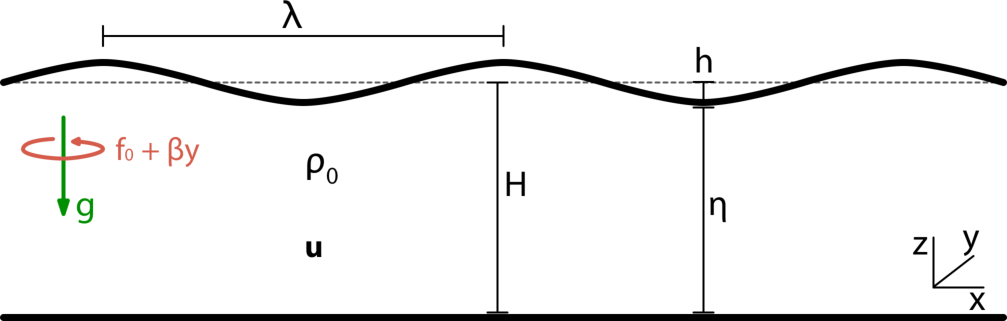
\includegraphics{shallow_water}
    \caption{The Shallow Water Configuration}
    \label{fig:shallow}
  \end{marginfigure}
  The equations being solved are
  \begin{subequations}
    \label{eqn:sw}
    \begin{align}
      \dd{u}{t} - fv &= - g \dd{h}{x} \\
      \dd{v}{t} + fu &= - g \dd{h}{y} \\
      \dd{h}{t} + H(\dd{u}{x} + \dd{v}{y}) &= 0
    \end{align}
  \end{subequations}
  where fluid height $\eta = H + h$, $g$ is gravity, and Coriolis parameter is $f=f_0 + \beta y$.

  The partial derivatives in space are approximated by a first-order central
  difference method and timestepping is performed using a linear-multistep method,
  the three-step Adams-Bashforth method.
  Appendix A \ref{sec:appendixa} details the numerical methods used.

  The code can be run on either Python 2 or Python 3, the only additional requirements are the libraries \texttt{numpy} and \texttt{matplotlib}.
  If you have not used Python on your computer before, you are unsure if you have the libraries, or if it's just been a long time since you used Python I recommend using one of the scientific distributions that are available to download.

  The two main choices are Enthought Canopy and Contiuum Anaconda.
  I use and recommend Anaconda; installing the latest version from the Continuum website \footnote{\url{https://www.continuum.io/downloads}} will give you the latest release of Python along with the most popular libraries \footnote{Notably \texttt{numpy}, \texttt{scipy}, \texttt{pandas}, \texttt{matplotlib}, \texttt{sympy} and \texttt{ipython}.  These six libraries will solve 99\% of your numerical, statistical and dataprocessing needs.
  A full list of included packages can be found at \url{http://docs.continuum.io/anaconda/pkg-docs}.}.
  Once the installer has been run, open a new terminal or command prompt window and you should have access to the new version of Python.

  A standard text editor such a Notepad is all that is required to edit the code, but not a \emph{word processor} like Microsoft Word.
  While Notepad is sufficient, there are many more powerful text editors available that make writing code a much more pleasant experience.
  Atom  \footnote{\url{https://atom.io/}} is a free, cross-platform option text editor with good support for Python.

  \section{Experiments}
  \label{sec:Experiments}

  \subsection{Experiment 1: Geostrophic Balance in 1-D}
  \label{sub:exp1}

  An introduction to the code.  By the end you will have run an example of geostrophic adjustment in one dimension and have an understanding of how the code can be changed.

  The first experiment demonstrates geostrophic adjustment in one dimension.
  There is no variation in the y-direction; the system that is being modelled is
  \begin{subequations}
    \begin{align}
      \dd{u}{t} &= fv - g \dd{h}{x} \\
      \dd{v}{t} &= -fu \\
      \dd{h}{t} &= -  H\dd{u}{x}
    \end{align}
  \end{subequations}
  Given some initial conditions and sensible values for $g$, $H$ and $f$ the system will be solved numerically.
  The intial conditions and constants are set
  \begin{align*}
    L_x &= \num{2e7} & H &= \num{100} & f &= \num{1e-5} & g &= \num{1} \\
    u_0 &= 0  & v_0 &= 0 & h_0 &= \tanh(100 \cdot x / L_x)
  \end{align*}
  and the code is allowed to evolve in time, taking a timestep $\Delta t = 1000$.
  \marginnote[-4em]{The code does not assume any units, but here the choice of constants scales the problem to be in [m] and [s].}
  \begin{itemize}
    \item Download the python script \texttt{linearshallowwater.py} from the
    course website \footnote{\url{http://empslocal.ex.ac.uk/people/staff/gv219/ecmm719/index.html}}.
    \textbf{If at any point you have changed several things, something goes really wrong and you can't get the code to run anymore, just go back to the course website and download a new copy.  You are encouraged to experiment and try new things!}
    \item Open a terminal (Mac/Linux) or command prompt (Windows), change directory to the location of the saved file and run it with the \texttt{python} command.
    \begin{minted}[mathescape]{bash}
      $ cd Downloads
      $ python linearshallowwater.py
    \end{minted}
    \begin{marginfigure}
      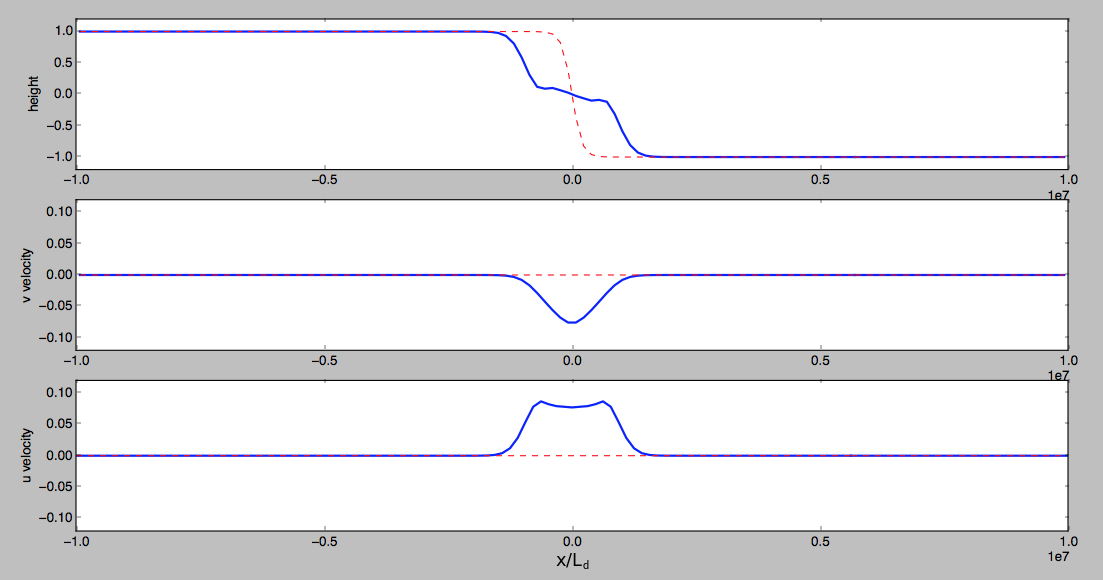
\includegraphics{geostrophy}
      \caption{A stepped height field undergoing geostrophic adjustment.}
      \label{fig:1dgeo}
    \end{marginfigure}
    \item The code should begin to run and an animation window will appear (Figure \ref{fig:1dgeo}).  If you can't see the chart check:
    \begin{itemize}
      \item That it is not hidden behind another window.  Sometimes the python plotting window can be opened behind your terminal or text editor window.
      \item That there are no errors on the command line.  If there are and you're not sure how to fix them, let me know.
    \end{itemize}
    \item Once you've got the code running, try changing some of the constants and see what happens.
    \begin{itemize}
      \item Set $f \gg \num{1e-5}$ and $f = \num{0.0}$.
      \begin{enumerate}
        \item What is happening in each of these cases?
        \item What happens to the gravity waves that radiate outwards?
        \item What is the problem with this numerical model compared with the analytic solution? \emph{Hint: boundary conditions.}
      \end{enumerate}
      \item If you want to see the simulation run longer, increase \texttt{nsteps} (found at around line \texttt{414}).
      \item (Advanced) The initial conditions for this experiment are set around line \texttt{315}.
      Try using a condition
      \begin{equation*}
        h_0 = \cos^n(\pi \cdot x / L_x)
      \end{equation*}
      where you can increase $n$ to get a more isolated hump.
    \end{itemize}
  \end{itemize}


  \subsection{Experiment 2: Geostrophic Adjustment in 2-D}
  \label{sub:exp2}
  We'll now consider the two-dimensional case where derivatives $\dd{}{y} \ne 0$ in general.
  So the system (\ref{eqn:sw}) will be solved in full.
  \begin{itemize}
    \item Make the following changes and run the code from the command line.
    \begin{minted}{python}
experiment = '2d'    # line 32
f0 = 0.0             # line 49
    \end{minted}
    \item You should see the case for a non-rotating fluid begin to run on
    your screen.  The height field is set with an initial condition of a small
    gaussian added to one point in the field.  As the equations evolve $u$ and
    $v$ velocities are induced and gravity waves radiate outwards from the initial disturbance.
    \begin{enumerate}
      \item Where on the Earth is $f_0 = 0$?
      \item (Advanced) What speed do you expect the gravity waves to be propagating at in this model?
    \end{enumerate}
    \begin{marginfigure}
      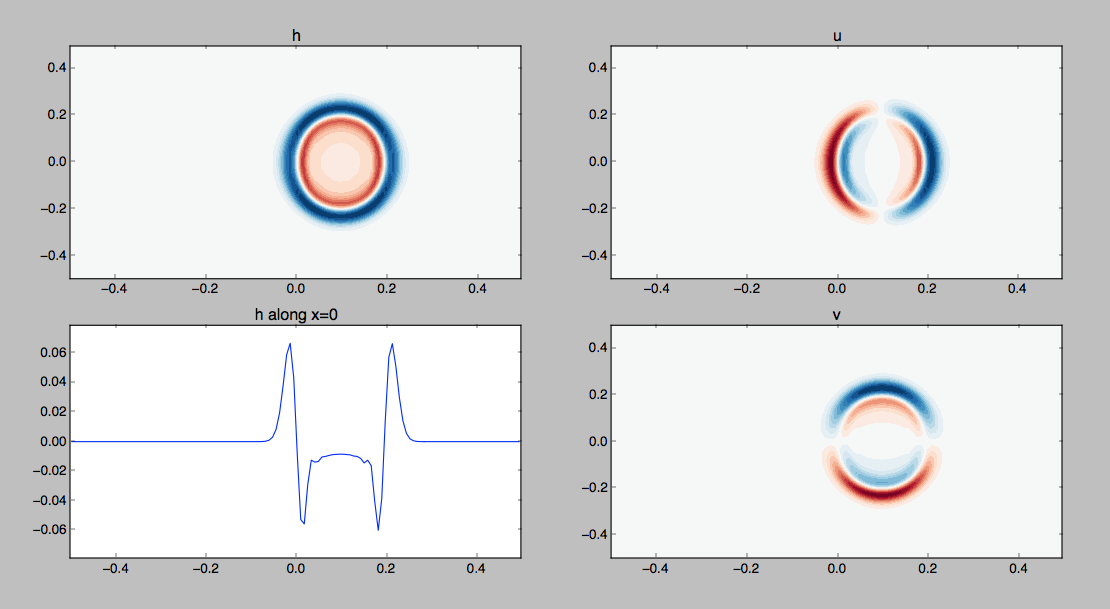
\includegraphics{gravity_waves}
      \caption{Gravity waves propagating away from an initial disturbance.}
      \label{fig:gravwaves}
    \end{marginfigure}
    \item Now try changing the Coriolis parameter to be something similar to that experienced in the mid-latitudes.
    \begin{enumerate}
      \item Change the value of $f_0$ back to $\num{1e-5}$ and rerun the two-dimensional case to compare with the irrotational version.
      \begin{enumerate}
        \item What happens to the gravity waves?
        \item What happens to the initial condition?
      \end{enumerate}
      \item Increase $f_0$ further.  What happens to the amplitude of the gravity waves as $f_0$ increases?
    \end{enumerate}
  \end{itemize}

\subsection{Advanced Experiments}
\label{sub:advanced}
  The code is quite versatile and capable of creating some other interesting dynamics.
  Here are a few more experiments you can try.
  These examples go beyond the scope of ECMM719; if you are interested further information of equatorial waves can be found in the Second Edition material for the Atmospheric and Oceanic Fluid Dynamics book under the section \emph{Waves on the Equatorial Beta Plane} \cite{Vallis:2015wb}.
    \begin{itemize}
      \item Coastal Kelvin Waves on the East Pacific coast.
      \begin{minted}{python}
Ly = 2.0e7                    # line 42
boundary_condition = 'walls'  # line 44
f0 = 0.0                      # line 49
beta =  2.0e-11               # line 50
      \end{minted}
      You may need to increase \texttt{nsteps} to see a longer simulation.

      As the initial height field decays, an \emph{equatorial Kelvin wave} moves Eastward.  When it reaches the boundary, it becomes a \emph{coastal Kelvin wave}.
    \item Equatorial Kelvin and Rossby waves.
          \begin{minted}{python}
boundary_condition = 'periodic'   # line 44
f0 = 0.0                          # line 49
beta =  2.0e-11                   # line 50
gr =  1.5e6                       # line 310
          \end{minted}
        \texttt{gr} specifies the radius of the disturbance in the height field.
        Here it is made bigger to be of order of the \emph{Rossby Deformation Radius} $L_d = \frac{\sqrt{gH}}{\beta}$.
      An equatorial Kelvin wave travels eastward along the equator, while two, slower moving, Rossby waves move westward in the tropics.
    \end{itemize}

  \section{Appendix A: Numerics}
  \label{sec:appendixa}

  \noindent This is a \emph{very} brief overview of the numerics used to implement the model.
  If you are interested in learning more about numerical methods in GFD, Dale Durran's book is an excellent resource \cite{Durran:2010hy}.

  If you are interested in using this code to model a specific problem, there is an up-to-date customisable version online \footnote{\url{https://github.com/jamesp/shallowwater}}.
  This repository has both the linear model and a fully nonlinear model of the shallow water equations.

  \noindent The model implemented here uses finite difference methods to calculate the derivatives in the spatial dimension and the Adams-Bashforth three-step method to integrate forward in time.

  \subsection{Spatial Derivatives}
  \label{sub:spatialderivatives}
  For a continuous function $u(x)$ the definition of a derivative is
  \begin{equation}
    \label{}
    \dd{u}{x} = \lim_{\Delta x \to 0} \frac{u(x - \Delta x) - u(x + \Delta x)}{2 \Delta x}
  \end{equation}
  As computers cannot deal with smooth functions exactly, the domain must be discretised into a finite number of \emph{nodes}.
  These nodes are denoted $x_j$ and spaced equally $\Delta x$ apart.
  Denote the value of $u_j = u(x_j)$ then the derivative at point $x_j$ can be approximated by considering only the values of $u$ at nodes:
  \begin{equation}
    \label{eq:cendiff}
    \dd{u_j}{x} \simeq \frac{u_{j+1} - u_{j-1}}{2 \Delta x}
  \end{equation}
  This is the \emph{central difference} method of calculating a spatial derivative and is used extensively in this model.
  \begin{marginfigure}
    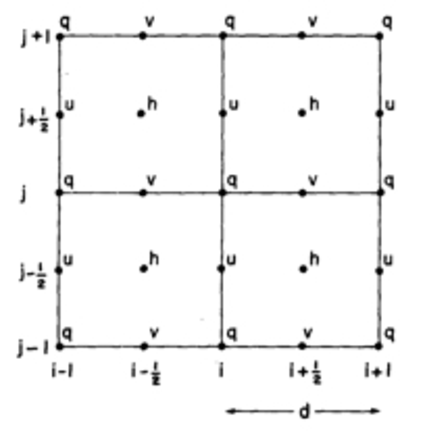
\includegraphics{cgrid}
    \caption{The Arakawa-C grid. From \citep{Arakawa:1981bx}}
    \label{fig:cgrid}
  \end{marginfigure}
  Clearly, an error has been introduced here for any function other than a
  straight line, the error is proportional to $\Delta x$.
  If $\Delta x$ is reduced, error will be reduced but computing time will be
  increased as to calculate the value of $u(x)$ across the domain requires
  calculating the value at more nodes.
  The central-difference equation (\ref{eq:cendiff}) has a weakness - it is
  performed over a distance of $2 \Delta x$ and the new value at $u_i$ is
  decoupled from the previous value at $u_i$ as it depends solely on
  values at neighbouring nodes.

  For improved numerical stability, the locations of $u$, $v$ and $h$ values are staggered in a configuration known as the \emph{Arakawa-C grid} (Figure~\ref{fig:cgrid}).
  This distribution of value nodes means that, for example, the central difference approximation
  \begin{equation}
    \dd{h}{x} \simeq \frac{h_{i+1/2} - h_{i-1/2}}{\Delta x}
  \end{equation}
  falls at the location of the $u_i$ node.
  In the linearised shallow water equations this is a desirable property:
  the value of $u$ at the next timestep depends on $\dd{h}{x}$ and using
  the staggered configuration the dependency is on immediately adjacent values
  over a distance of $\Delta x$.

  \subsection{Time Derivatives}
  \label{sub:timederiv}

  In simulating the shallow water equations we are essentially solving
  an initial value problem.
  Once the spatial derviatives have been approximated the equations can
  be stepped forward in time.
  The linear momentum equation can be discretised
  \begin{equation}
    \frac{u_j^{(n+1)} - u_j^{(n)}}{\Delta t} - fv_j^{(n)} = - \frac{\phi_{j+1}^{(n)} - \phi_{j-1}^{(n)}}{2 \Delta x}
  \end{equation}
  where $^{(n+1)}$ denotes the index in time in the same way $_j$ denotes
  index in space.

  This can be rearranged to calculate the value of $u_j^{(n+1)}$ entirely in
  terms of variables at the $^{(n)}$ time-level.
  \begin{equation}
    u_j^{(n+1)} = u_j^{(n)} + {\Delta t}
      \left( fv_j^{(n)} - \frac{\phi_{j+1}^{(n)} - \phi_{j-1}^{(n)}}{2 \Delta x} \right)
  \end{equation}
  Timestepping in this manner is known as \emph{Euler's method}.
  This is an \emph{explicit} numerical scheme as the value at time $^{(n+1)}$
  depends solely on values at $^{(n)}$.

  Euler's method is the simplest possible timestepping procedure,
  for better accuracy here the slightly more complicated three-step \emph{Adams-Bashforth}
  method is used for timestepping.  Adams-Bashforth $n$-step routines are a family
  of \emph{linear multistep} methods that calculate the state at the next timestep
  based on a weighted average of the states at the previous $n$ time levels.

  For a differential equation of the form $ \diff{y}{t} = f(t, y) $ the
  first three Adams-Bashforth multistep methods are
  \begin{align*}
    y_{n+1} &= y_n + \Delta t f(t_n, y_n)  \\
    y_{n+2} &= y_{n+1} + \Delta t \left( \frac{3}{2}f(t_{n+1}, y_{n+1}) - \frac{1}{2}f(t_n, y_n) \right) \\
    y_{n+3} &= y_{n+2} + \Delta t \left( \frac{23}{12} f(t_{n+2}, y_{n+2}) - \frac{4}{3} f(t_{n+1}, y_{n+1}) + \frac{5}{12}f(t_n, y_n)\right) \\
  \end{align*}

\bibliography{biblio}
\bibliographystyle{plainnat}

\end{document}
